
\chapter{Emergent biaxial order in hybrid chiral LCs}
\chaptermark{Hybrid LCs: single-particle effects}


\begin{abstract}
Cholesteric liquid crystals (LCs) are classic examples of complex chiral mesophases with long-ranged periodicity but lack positional order at large length scales. Doping molecular cholesterics LCs with thin colloidal rods or disks with a large  length-to-width ratio adds a further a further level of complexity due to the interplay between weak surface anchoring forces and elastic distortions around the rod-LC interface. We demonstrate that the rods have a strong tendency to orient perpendicular to the helix axis and local director, thus imparting strong local biaxiality on the hybrid cholesteric structure. We theoretically argue that the splay-bend elastic anisotropy plays a key role in stabilizing local orthorhombic order along the helix.  Our predictions are corroborated by experimental results obtained in the group of I. Smalyukh (University of Colorado, USA) that we briefly review. We also discuss the case of discs and find a similar scenario of anomalous biaxial order along the helical director for discs with homeotropic anchoring immersed in short-pitch cholesteric hosts LCs. 


\end{abstract}



\section{Introduction}

% TODO: write introduction (inspired by Smalyukh's?)


Since the experimental discovery of chiral nematic liquid crystals (LCs) over 150 years ago \cite{planer1861notiz,reinitzer1888beitrage}, LC mesophases featuring chirality and long-range orientational order have been the focus of many research studies. The fundamental studies of geometry and topology of chiral nematic LCs as model systems provide extensive insights into physics principles associated with experimentally less accessible systems like particle physics or cosmology \cite{wu2022hopfions}, in addition to their technological application in electro-optics and displays. On the other hand, biaxial nematic mesophases have been highly sought-after in soft matter systems since their first theoretical consideration in 1970 \cite{freiser1970ordered}. However, even in a soft-matter system with strongly biaxial building blocks such as brick-shaped molecules, biaxiality was experimentally elusive and hard to unambiguously demonstrate in equilibrium states. Recent reports of the experimental discovery of biaxial nematic order include observations in micellar and molecular LCs formed by amphiphilic and bent-core molecules, respectively \cite{yu1980observation,tschierske2010biaxial}, and also colloidal dispersion of highly anisotropic particles immersed in molecular LC hosts, so-called hybrid nematics \cite{liu2016,mundoor2021,mundoor2018}.
The interplay between chirality and biaxiality in orientational order has been intensively studied for LC systems \cite{priest1974biaxial,kroin1989chirality,bunning1986effect,harris1997microscopic,dussi2016entropy,dhakal2011chirality,longa1994biaxiality,canevari2015biaxiality}. It has been concluded that cholesteric twisted alignment and biaxial order of LC molecules amplify each other and that a chiral twist configuration cannot be observed without building blocks featuring a certain degree of biaxiality in their orientational distributions at the molecular level. However, for purely molecular systems, the chirality-enhanced biaxiality of the molecular distribution was predicted and experimentally found to be rather weak \cite{priest1974biaxial,kroin1989chirality,bunning1986effect,harris1997microscopic,dussi2016entropy,dhakal2011chirality,longa1994biaxiality,canevari2015biaxiality}, scaling as $\ (qL_{\rm m})^2$ according to the prediction by Priest and Lubensky for single-component molecular LCs \cite{priest1974biaxial} (here $q=2\pi/p$, $p$ is the pitch of the chiral nematic and $L_m$ the molecular length). To date, to the best of our knowledge, there are no experimental or theoretical considerations of how the biaxiality of the orientational distribution of anisotropic colloidal particles could interplay with the chirality of the nematic host in hybrid molecular-colloidal LC systems.  



\begin{figure}
	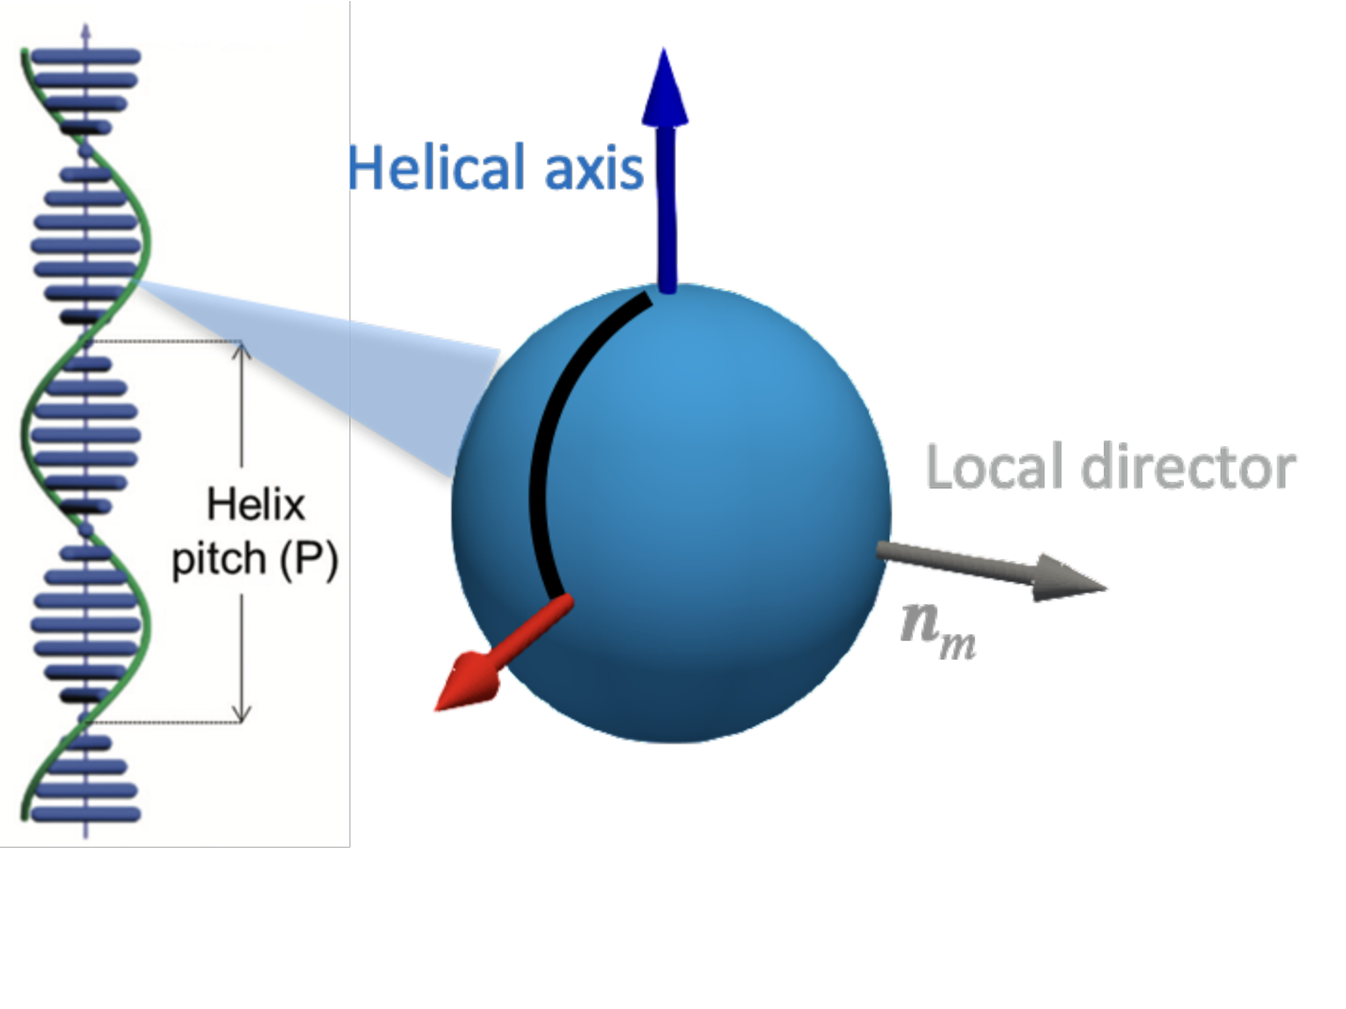
\includegraphics[width = 0.6 \columnwidth]{figures/chapter-3/tripod}
	\caption{ Illustration of alignment opportunities for an anisotropic colloidal particles immersed in a cholesteric host LC. Depending on the surface anchoring properties of the colloid  and pitch of the cholesteric host, the colloid may  preferentially  align along either of the three main directions of the tripod.   Alignment along the red arrow leads to strong emergent local biaxial order of a hybrid colloidal-molecular LC.  }
	\label{tripod}
\end{figure}



In this chapter we present a theoretical survey of ordering properties of colloidal particles immersed in a low-molecular weight liquid crystal. Based on a simple mean-field theory that accounts for the surface anchoring energy of a single colloid we explore the alignment properties of thin elongated rods and flat discs with respect to the helical director field of the molecular host fluid 
(see \fig{twisdis}).  A key element is the preferred surface anchoring  properties of the molecular LC at the colloid surface which opens op several distinctly different ordering scenarios. Specific symmetries  that we explore  here are homeotropic, planar (see \fig{surfancho}) as well as conically degenerate surface anchoring for the case of discs.   Comparing with recent experimental results obtained in the group of I. Smalyukh (University of  Colorado, USA) we conclude that our theory accounts for most of the experimental observations, but for one case. We demonstrate that the alignment of rodlike colloid with homeotropic anchoring is not  driven by weak surface anchoring forces, but rather by a twisted surface disclination effects.  We address the weak elastic deformations around the colloids and demonstrate the twisted disclination wrapped around a thin rod  is the main driving forces between hometropic rods aligning perpendicular to the local host director and helical axis, thus imparting strong biaxial order onto the hybrid LC. A similar scenarios is envisaged for homeotropic discs, bit only in strongly cholesteric hosts with a pitch comparable to the disc diameter.




\section[Surface anchoring of a cylindrical rod]{Surface anchoring of a cylindrical rod immersed in a cholesteric host}


\begin{figure}
	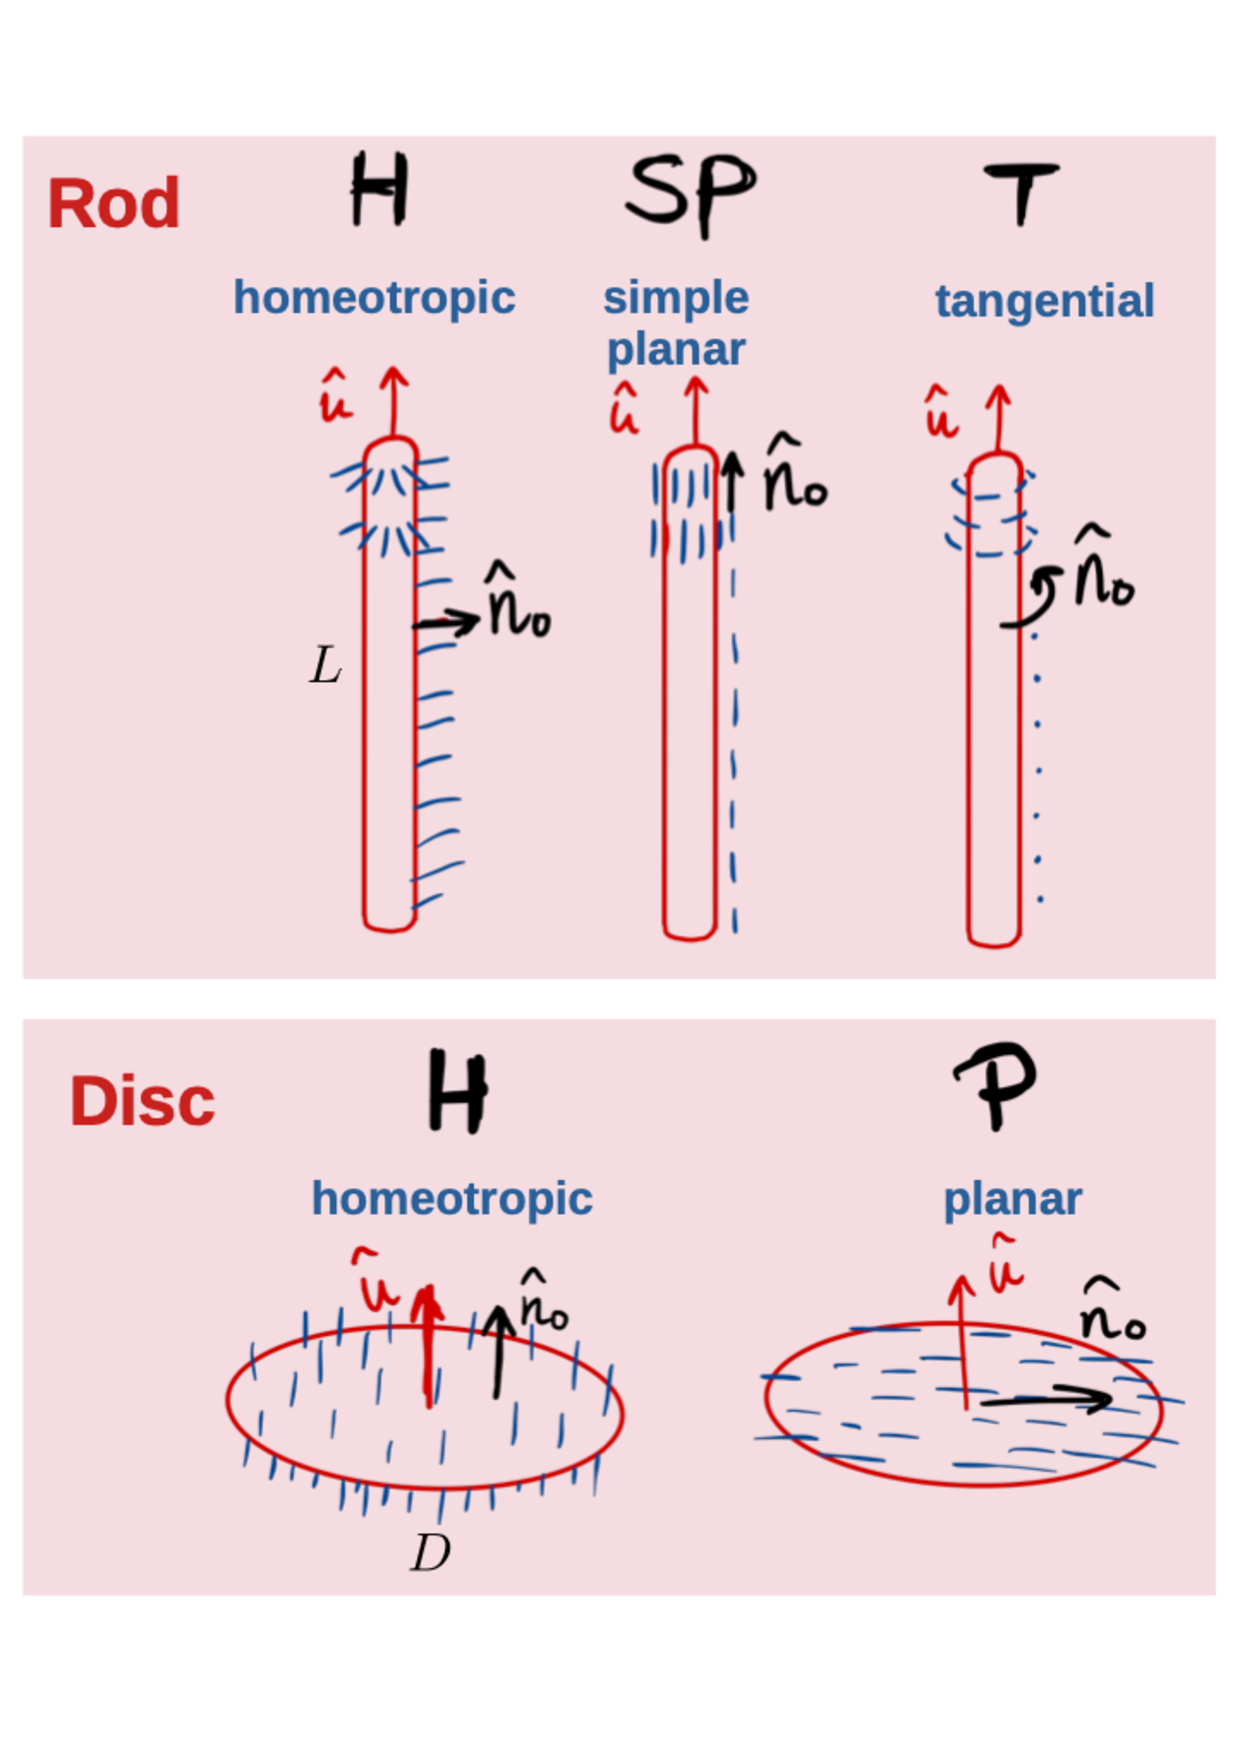
\includegraphics[width = 0.6 \columnwidth]{figures/chapter-3/surfanchoring}
	\caption{ Illustration of the different surface anchoring scenarios for a colloid rod with length $L$ (top) and disc with diameter $D$ (bottom).  }
	\label{surfancho}
\end{figure}





Let us consider a low-molecular-weight chiral liquid crystal (such as 5CB with chiral dopants) with a director field $\bn(z)$ twisted along $Z$-axis of a Cartesian laboratory frame. The director field of the cholesteric solvent, denoted by ``$s$",  may be parameterized as:
\beq
\bn_{s}(z) = \bx \cos q Z  + \by \sin q Z
\label{ns}
\eeq
in terms of the pitch  $p = 2 \pi/q$ and handedness $q>0$ that we assume right-handed without loss of generality.
Next, we immerse a infinitely thin cylindrical rod with aspect ratio $L/D \rightarrow \infty$ into the chiral nematic  phase. The main axis of each rod can be parameterized as $\bhu = \bx \sin \theta \sin \varphi + \by \sin \theta \cos \varphi + \bz \cos \theta $ in terms of a polar $\theta$ and azimuthal angle $\varphi$ with respect to the helical axis $\bz$. The presence of the rod will generate elastic distortions of the uniform director field $\bn_{s}(\bfr)$ due to the specific anchoring of the molecules at the surface of the rod, quantified by  the surface anchoring energy  $W_{0}>0$ (units energy surface area). The extent of elastic deformation around the colloid surface ratio is commonly indicated by the surface extrapolation length $\ell_{s} = K/W_{0}$ where $K$ designates the typical elastic constant of the thermotropic liquid crystal.   In this project we focus on  the regime of large surface extrapolation length $ ( \ell_{s} \rightarrow \infty )$, in which case the elastic distortions are infinitesimally weak and the main energetic contribution imparted by the rod inclusions stems from the surface anchoring energy. Elastic corrections will be accounted for later on.   If we assume the molecular director field  $\bn$ to remain completely undistorted,  the surface anchoring free energy can be obtain from a simple Rapini-Papoular integral of \eq{ns} over the colloid surface denoted by ${\mathcal S}$:
\beq
F_{s} = -\frac{1}{2} W_{0} \oint d{\mathcal S}  (\bn_{s} \cdot \bn_{0}({\mathcal S}))^{2}
\label{rapo}
\eeq
with $\bn_{0}$ represent a unit vector normal to the colloid surface in case of {\em homeotropic} anchoring and tangential to the surface if the anchoring is {\em planar}.


For the particular case of a thin cylinder, we shall neglect small contributions associated with the ends of the cylinder so we only need to parameterize the cylindrical surface of magnitude $\pi LD$ following the principal contour $\bfr_{{\mathcal S}}(t) = \bfr_{0} +  \frac{L}{2}t\bhu $
with $-1<t<1$ of a cylinder with centre-of-mass $\bfr_{0}$. The surface anchoring free energy then becomes:
\beq
F_{s} = -\frac{1}{8} LDW_{0} \int_{0}^{2 \pi} d \phi  \int_{-1}^{1} dt  [ \bn_{s}( \bfr_{{\mathcal S}} \cdot {\bf \hat{z}}  ) \cdot \bn_{0} ]^{2}
\label{usurf}
\eeq
In order to describe various anchoring situations  we define two unit vectors $\bhe_{1,2}$ orthogonal to $\bhu$ and parameterize [Brochard-DeGennes]:
\beq
\bn_{0} = \begin{cases}
      \bhe_{1} \cos \phi + \bhe_{2} \sin \phi &  \textrm{H} \\
         -\bhe_{1} \sin \phi + \bhe_{2} \cos \phi &  \textrm{T} \\
      \bhu & \textrm{SP}
   \end{cases}
      \label{plahom}
\eeq
In the case of homeotropic (H) anchoring  the molecular director favors perpendicular alignment to the cylindrical surface, whereas  for tangential (T)  anchoring the easy axis follows the circular perimeter of the cylindrical cross section.
 The simple planar (SP) case corresponds to the easy axis $\bn_{0}$ pointing along main rod direction.    We obtain the following generic expression:
\begin{align}
 F_{s} = -\frac{\pi}{8} LDW_{0} \left ( w_{1} + w_{2} \cos (2 \delta )  \frac{\sin (qL \cos \theta)}{qL} \right )
 \label{us}
\end{align}
with $\delta = \varphi - q Z$ the azimuthal angle along a particle frame co-rotating with the  helical director so that $ \int d \bhu = \int_{0}^{2 \pi} d \delta \int_{-1}^{1}  d ( \cos \theta )$  and $w_{1}$ and $w_{2}$ are angle-dependent coefficients that depend on the particular anchoring situation:
\beq
w_{1} = \begin{cases}
      (1+ \cos^{2} \theta)  &  \textrm{H/T} \\
    2   \sin ^{2} \theta  & \textrm{SP}
   \end{cases}
      \label{w1}
\eeq
and
\beq
w_{2} = \begin{cases}
    -  \sin \theta \tan \theta    &  \textrm{H/T} \\
    2  \sin \theta \tan \theta   & \textrm{SP}
   \end{cases}
      \label{w2}
\eeq
in terms of the polar $\theta$ and azimuthal rod angle $\varphi$ with respect to the  helical axis. Note that the surface anchoring free energy is the same for the homeotropic and tangential anchoring scenarios.


For the homeotropic (H) case the free energy is minimal when  $\theta^{\ast} = 0$  (with the azimuthal angle $\varphi$ randomly distributed) which corresponds to the rod being  aligned along the helical axis. However, there is a second, degenerate minimum at $\theta^{\ast} = \pi/2$ and $\delta^{\ast} = \pi/2$, that describes a  rod pointing perpendicular both to the helical axis {\em  and} the local director.  The minimum surface anchoring energy is $F_{s} = -(\pi/4) LD W_{0}$ for both cases.  The energy barrier between the two minima is only about 0.2 $k_{B}T$ per rod so thermal fluctuations should easily make  the colloids switch from one state to the other.
 For simple planar (SP) anchoring we only find a single minimum at $\theta^{\ast} = \pi/2$ and $\delta^{\ast} = 0 $, i.e., the rod preferentially aligns along the revolving local nematic director.



\subsection{Non-interacting rods}

By balancing the surface anchoring free energy with the orientational entropy of the individual rods we easily establish the angular probability through the Boltzmann distribution:
  \beq
  f( \bhu ) = \mathcal{N} \exp (- \beta F_{s} (\delta, \theta)  )
  \label{fsingle}
  \eeq
 with $\beta^{-1} = k_{B}T$ the thermal energy in terms of temperature $T$ and Boltzmann's constant $k_{B}$ and $\mathcal{N}$ a normalization constant ensuring that $\int d \bhu f(\bhu) = 1$.  The surface anchoring strength is expressed  in dimensionless form by $\bar{w} = \beta LDW_{0}$.  The distributions are visualized in \fig{frod}.
It is easy to infer from \eq{us} that the polar and azimuthal angles are strongly coupled. This indicates that the local distribution of rod orientations around the principal alignment directions (blue, red or white arrow in \fig{frod}) is rendered {\em biaxial} by the chiral twist, as expected.  The most interesting situation arises for the H/T case where there is a subpopulation of  rods aligned along the helical axis ($qL=1$). In order to gain further insight into the orientational symmetry of those rods, we perform a small-angle expansion around   $\theta_{e} = 0$ and retain the leading order coupling term between the two principal angles $\theta$ and $\delta$. The angular fluctuations about the helical axis (blue) are then described by the following free energy
\beq
F_{s} \approx \frac{\pi}{8} LDW_{0}  j_{0}(qL) \cos (2 \delta) \theta^{2}
\label{ht_fluc_new}
\eeq
with $j_{0}(x) = \sin (x)/x$. It suggests that the subpopulation of rods aligned along the helical axis in fact adopt a {\em twist-bend}-type organization with a pitch $q$ identical to that of the molecular host. Contrary to cholesterics, these phases are characterized by a nematic director co-aligning with the helical axis. However, the situation here is more subtle given that  chirality is only manifested at the level of orientational fluctuations around a mean director ``backbone" that itself is not chiral.   We  identify a further interesting feature; depending on the sign of $j_{0}(qL)$ the twist-bend helix may be either in phase with the molecular helix ($\delta^{\ast} =0$ for  $qL=4$) or out-of-phase ($\delta^{\ast} = \pi/2$ for $qL=2$).


  \begin{figure}
	\includegraphics[width = 0.8\columnwidth]{figures/chapter-3/frod}
	\caption{ Unit-sphere projections of the local orientational probability of a rod immersed in a low molecular-weight cholesteric phase at different surface anchoring strengths $\bar{w} = \beta W_{0}LD$. Zones of high orientational probability are in red.  A bistable distribution is found for the homeotropic/tangential (H/T) anchoring case at elevated anchoring strength. For all distributions, the rod-length-to-pitch is $qL=1$. }
	\label{frod}
\end{figure}


%Finally, we may probe the possibility of {\em tetragonal} nematic order ($D_{4h}$) with four-fold symmetry across the plane perpendicular to the cholesteric director ${\bf \hat{n}}_{s}$. We propose the following order parameter:
%\beq
%\Delta_{4} = \langle (a^{2} - b^{2})^{2} - a^{2}b^{2} \rangle_{f_{q}}
%\eeq
%We may thus identify the local nematic symmetry of the colloids, namely  uniaxial  ($S \neq 0, \Delta = 0, \Delta_{4} =0$),  orthorhombic biaxial ($S \neq 0, \Delta \neq 0, \Delta_{4} \neq 0$) or tetragonal  ($S \neq 0, \Delta = 0, \Delta_{4} \neq 0$).
%}


\subsection{Non-interacting discs}

We may now explore the case of a  thin disc with $L \ll D$ immersed in a cholesteric LC. Let us denote its normal by $\bhu$ and ignore anchoring at the rim. Similar to the case of rods we  consider homeotropic (H) and planar (P)  anchoring symmetries that we may express as follows:
\beq
\bn_{0} = \begin{cases}
      \bhu & \textrm{H} \\
      \bhe_{1} \cos \xi + \bhe_{2} \sin \xi &  \textrm{P} \\
       \end{cases}
      \label{plahomm}
\eeq
The angle $0 < \xi < 2 \pi$ must be chosen randomly in the case when  planar anchoring is degenerate across all direction on the disc surface.
Ignoring finite-thickness effects for $L \ll D$ we parameterize the face of the disc  as follows:
\beq
\bfr_{{\mathcal S}} = \bfr_{0} + \frac{D}{2} t [\bhe_{1} \sin \phi + \bhe_{2}\cos \phi ]
\eeq
with $0< t <1 $ and $0 < \phi < 2 \pi$.
The surface anchoring energy per disc face is expressed analogous to \eq{usurf}:
\begin{align}
F_{s} &= -\frac{1}{4}  W_{0} D^{2} \int_{0}^{2 \pi} d \phi   \int_{0}^{1} dt t \int_{0}^{2 \pi} \frac{d \xi}{2 \pi} [ \bn_{s}( \bfr_{{\mathcal S}} \cdot {\bf z} ) \cdot \bn_{0} ]^{2}
\label{usurf2}
\end{align}
Leading to the following generic expression:
\begin{align}
 F_{s} = -\frac{\pi}{4}  W_{0}D^{2} \left ( w_{1} + w_{2} \cos (2 \delta ) \frac{J_{1}(qD | \sin \theta|)}{qD | \sin \theta| } \right )
 \label{usp}
\end{align}
with $J_{1}(x)$ a Bessel function of the first kind, $\delta = \varphi  - q z$ the  azimuthal angle with respect to the local cholesteric director, and coefficients:
\beq
w_{1} = \begin{cases}
    \frac{1}{2}  \sin ^{2} \theta    &  \textrm{H} \\
      \frac{1}{8}( 3 + \cos ( 2 \theta ))   & \textrm{P}
   \end{cases}
      \label{w1p}
\eeq
and
\beq
w_{2} = \begin{cases}
      \sin^{2} \theta    &  \textrm{H} \\
    -\frac{1}{2}  \sin^{2} \theta    & \textrm{P}
   \end{cases}
      \label{w2p}
\eeq
Similar to the rods the surface anchoring strength is expressed  in dimensionless form by $\bar{w} = \beta W_{0}D^{2}$. Taking discs with diameter $D \approx 2 \mu m$ and $W_{0} \approx 10^{-6} - 10^{-5} J/m^{2}$ we find an even higher value than for  the rods, namely  $\bar{w} \sim 10^{3}-10^{4}$ indicating that surface anchoring realignment is robust against thermal fluctuations.


   \begin{figure}
	\includegraphics[width = 0.8\columnwidth]{figures/chapter-3/fdisc}
	\caption{ Unit-sphere projections of the local orientational probability of a disc immersed in a low molecular-weight cholesteric phase at different surface anchoring strengths $\bar{w} = \beta W_{0}D^2$. For all distributions, the disc-diameter-to-pitch is $qD=1$. }
	\label{fd}
\end{figure}

\subsection{Conically degenerate surface anchoring}

The presented surface anchoring model is suitable for a vast selection of geometrical junctions between the cholesteric solvent and the particles. Another experimentally relevant scenario, and as a generalization of the previously evaluated situations, would consist of a preferred anchoring direction $\bn_{0}$ forming an angle $\alpha$ (and thus drawing a degenerate conical surface with apex angle $\alpha/2$) with respect to the vector normal to the colloid surface. Let $\xi$ be the integration angle around such a cone.

For rod-like particles, the anchoring free energy is expressed analogous to \eq{usurf}:
\begin{align}
F_{s} &= -\frac{1}{8} LDW_{0} \int_{0}^{2 \pi} d \phi   \int_{-1}^{1} dt \int_{0}^{2 \pi} \frac{d \xi}{2 \pi} [ \bn_{s}( \bfr_{{\mathcal S}} \cdot {\bf z} ) \cdot \bn_{0} ]^{2}
\end{align}
We may express $\bn_{0}$ in terms of the angles $\alpha$, $\phi$ and $\xi$:
 \begin{align}
\bn_{0} & = \bhe_{1}( \cos \phi \cos \alpha - \sin \phi \sin \alpha \cos \xi) \nonumber \\
       & + \bhe_{2} (\sin \phi \cos \alpha + \cos \phi \sin \alpha \cos \xi) \nonumber \\
       & + \bhu \sin \alpha \sin \xi
      \label{plahommm}
 \end{align}
Leading to an expression equivalent to \eq{us} with coefficients:
\beq
w_{1} =\frac{1}{2}(3 - \cos ^{2} \alpha + ( 3\cos ^{2} \alpha - 1 ) \cos ^{2} \theta )
\eeq
and
\beq
w_{2} = - \frac{1}{2}( 3\cos ^{2} \alpha - 1 ) \sin \theta \tan \theta
\eeq
We can similarly take \eq{usurf2} for discs. In this case we define $\bn_{0}$ as follows:
\beq
\bn_{0} = (\bhe_{1} \cos \xi + \bhe_{2} \sin \xi) \sin \alpha + \bhu \cos \alpha
      \label{plahommmm}
\eeq
Leading to an expression equivalent to \eq{usp} with coefficients:
\beq
w_{1} =\frac{1}{4}(2 - 2\cos ^{2} \alpha + ( 3\cos ^{2} \alpha - 1 ) \sin ^{2} \theta )
\eeq
and
\beq
w_{2} =\frac{1}{2}( 3\cos ^{2} \alpha - 1 ) \sin ^{2} \theta
\eeq
The corresponding distributions are given in \fig{fc}.

\red{TO BE INCLUDED}

\begin{figure}
	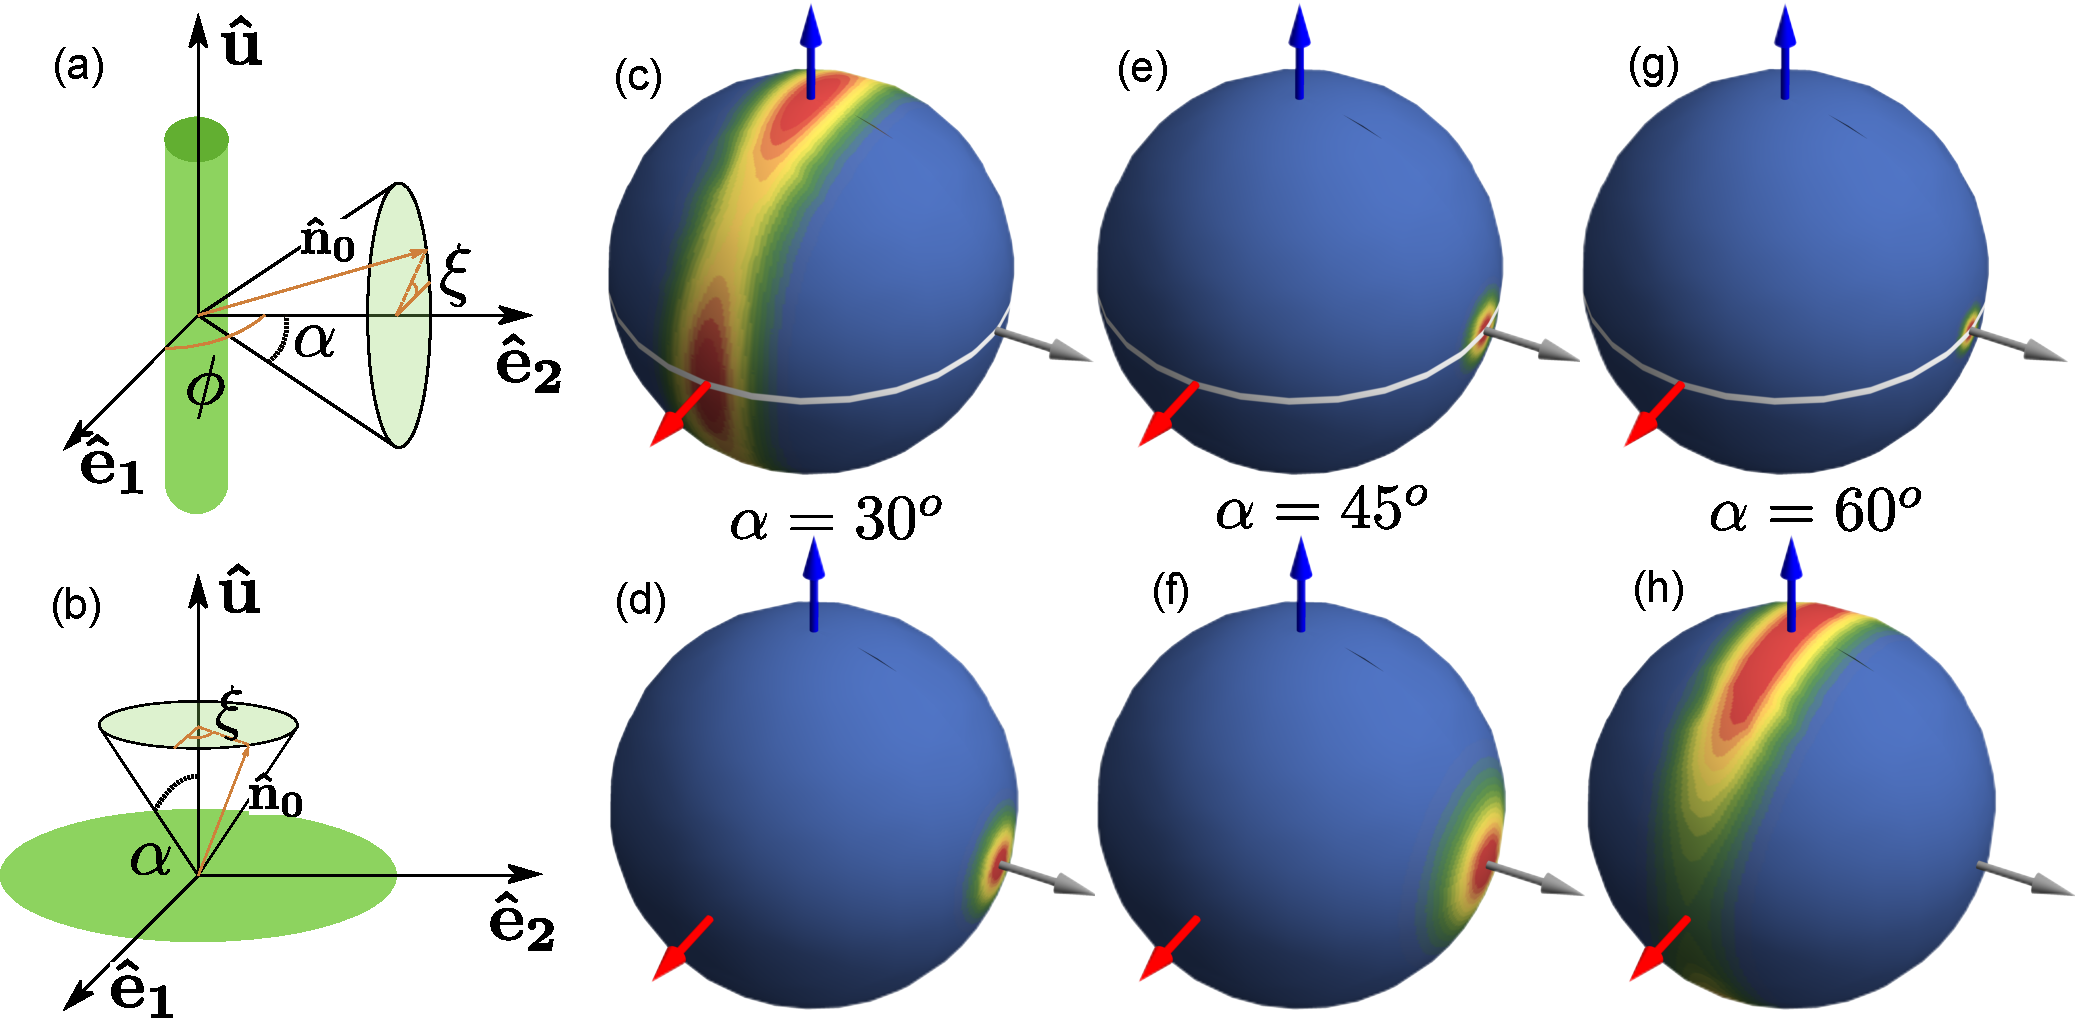
\includegraphics[width = \columnwidth]{figures/chapter-3/heliconical}
	\caption{ (a) (and (b)) Schemes to illustrate the conically degenerate surface anchoring with a fixed anchoring angle $\alpha$ on rods (and discs). (c-h) Unit-sphere projections of the local orientational probability of a rod (top panels c, e, g) or a disc (bottom panels d, f, h) immersed in a low molecular-weight cholesteric phase at different anchoring angles. For all distributions, the particle-length-to-pitch is $qL(D)=1$ and the surface anchoring strength is $\bar w = 100$. }
	\label{heliconical}
\end{figure}



\subsection{Order parameters}

In order to facilitate comparison with experimental results, we define orientational order  with respect to  $\bn_{s}$ which defines the principal direction of molecular alignment along the cholesteric helix. Taking the local host director $\bn_{s}$ as a reference we define a uniaxial order parameter:
\beq
S = \langle {\mathcal P}_{2} (\bhu \cdot \bn_{s})\rangle_{f_{q}}
\label{s2}
\eeq
A biaxial nematic order parameter measures the relative orientational order with respect to the principal directions orthogonal to $\bn_{s}$:
\beq
\Delta = \langle a^{2} - b^{2} \rangle_{f_{q}}
\label{d2}
\eeq
in terms of the projections $a= \bhu \cdot (\bn_{s} \times \bz)$ and $b = \bhu \cdot \bz$. We stress that this convention is by no means unique and one could also define orientational order from the tensor ${\bf Q}_{c} =  \frac{3}{2} \langle \bhu \otimes \bhu  \rangle_{f_{q}} - \frac{{\bf I}}{2} $ which measures the orientational order parameters ($S_{\rm c}$ and $\Delta_{\rm c}$) with respect to the principal colloidal alignment direction $\bn$, independent from the chosen reference frame.


\section[Model system]{Experimental model system}


The experiments performed in the group of I. Smalyukh are based on disk or rod-shaped $\beta- {\rm NaYF4:Yb/Er}$ particles are synthesized following the hydrothermal synthesis methods described in detail in Refs. \cite{mundoor2018,mundoor2021}. Homeotropic anchoring with 5CB (pentyl-cyanobiphenyl or 4-cyano-4'-pentylbiphenyl) molecules
on the $\beta-{\rm NaYF4:Yb/Er}$ disk surfaces is controlled
through surface-functionalization with a thin layer of
silica and polyethylene glycol.

The colloidal rods have length $L\approx 1.6 \mu m$, thickness $D \approx 25 nm$ and {\em homeotropic} (H) surface anchoring with amplitude $W_{0} \approx 10^{-5} J/m^{2}$. From this we find that $\bar{w} \approx 97$ indicating that the realigning forces generated by surface anchoring strongly exceed thermal fluctuation forces. The pitch of the cholesteric host is about $p \approx 30 \mu m $ so that $qL  \approx 0.335 $. The discs have a diameter of about $D \sim 2 \mu m $ and thickness of $L \sim 20 nm$. In view of their large diameter the surface anchoring amplitude $\bar{w} \sim 10^{3}-10^{4}$ each disk experiences strongly exceeds the thermal energy.  The results of the experiments are summarized in the table below. In additions, simulations have been performed based on numerically minmizing the Landau-DeGennes free energy around a colloidal particle immersed. The simulations fully account for the elastic anisotropy of the cholesteric host with input parameters based on the experimentally measured elastic moduli for 5CB. The surface anchoring amplitude and symmetry was varied in similar ways as in our theoretical approach.   Full details of the experiments and simulations will be disclosed in an upcoming joint publication with the group of I. Smalyukh. 



\begin{table}[h!]
\centering
    \begin{tabular}{|c||c c c c|} 
    \hline
    & $S$ & $\Delta$ & $S_{\rm{c}}$ & $\Delta_{\rm{c}}$ \\  
    \hline\hline
    homeotropic  disk &  0.6564 & 0.0673 & 0.6564 & 0.0673  \\ 
    \hline
    planar rod & 0.9360 & 0.0140 & 0.9360 & 0.0140   \\
    \hline
    homeotropic rod ($L = 1.7 \mu m$) &  -0.2561 & 0.7594 &  0.6976 & 0.1236  \\
    \hline
    homeotropic rod ($L = 3 \mu m$) & -0.3818 & 0.8935 & 0.8610 & 0.0650  \\
    \hline
    \end{tabular}
    \caption{Colloidal order parameters measured in the local molecular frame  and colloidal frame (with subscript `c') for each set of experiments. }
    \label{table_OPs}
\end{table}
From the measured order parameters  we infer that both  planar rods and hometropic discs both tend to align along the cholesteric director, whereas homeotropic rods strongly prefer to orient towards the perpendicular axis indicated in red in \fig{twisdis}. These obervations are in line with the distributions depicted in \fig{frod} for the rods and \fig{fd} for the discs. However, \fig{frod} suggests that hometropic rods with strong surface-anchoring coupling  $\bar{w} = 100 $ should  have an equal probability to the red and and blue arrows. This degeneracy is not observed in experiment where the subpopulation of rods pointing along the helix axis (blue) is estimated to be negligble. Clearly, the Rapini-Papoular surface anchoring energy does not suffice to explain the experimental observation which suggests that  elastic deformations incurred by the weak surface anchoring forces must play a subtle role.   This we will analyze next.


\section[Role of elastic distortions]{Comparison with experiments: role of elastic distortions}

In our analysis so far we have completely ignored elastic deformations of the host director ($\ell_{s} = K/W_{0} \rightarrow \infty$) so that rod realignment is dominated entirely by surface anchoring. The latter dictates that rods should point along the blue and red axis with equal probability (see \fig{frod}). The experimental reality, however, is that the surface anchoring extrapolation length is large but finite ($\ell_{s} \approx 600 nm \gg D$). Observations point at a scenario in which  rods  orienting along the red axis is largely preferred over the helical axis (blue). The reason why the latter is unfavorable  is that it involves a twisting of the surface disclination that runs along the rod contour which presumably costs energy. This is illustrated in \fig{twisdis}. No such twisting is necessary if the rod points along the red axis.   Clearly, the discrepancy between experiment and theory must be attributed to the  elastic distortions running along the rod surface (and their subsequent twisting) which was ignored in our model considerations thus far. In principle, weak director distortions may also lead to a minute decrease  of the bulk nematic order parameter,  in particular in regions where the director curvature is strong.  In our analysis, we will assume that the scalar order parameter of the host is preserved even close to the rod surface where director distortions are expected to be the strongest.



\subsection{Elastic energy of a twisted disclination wrapped around a thin rod}




\begin{figure}
	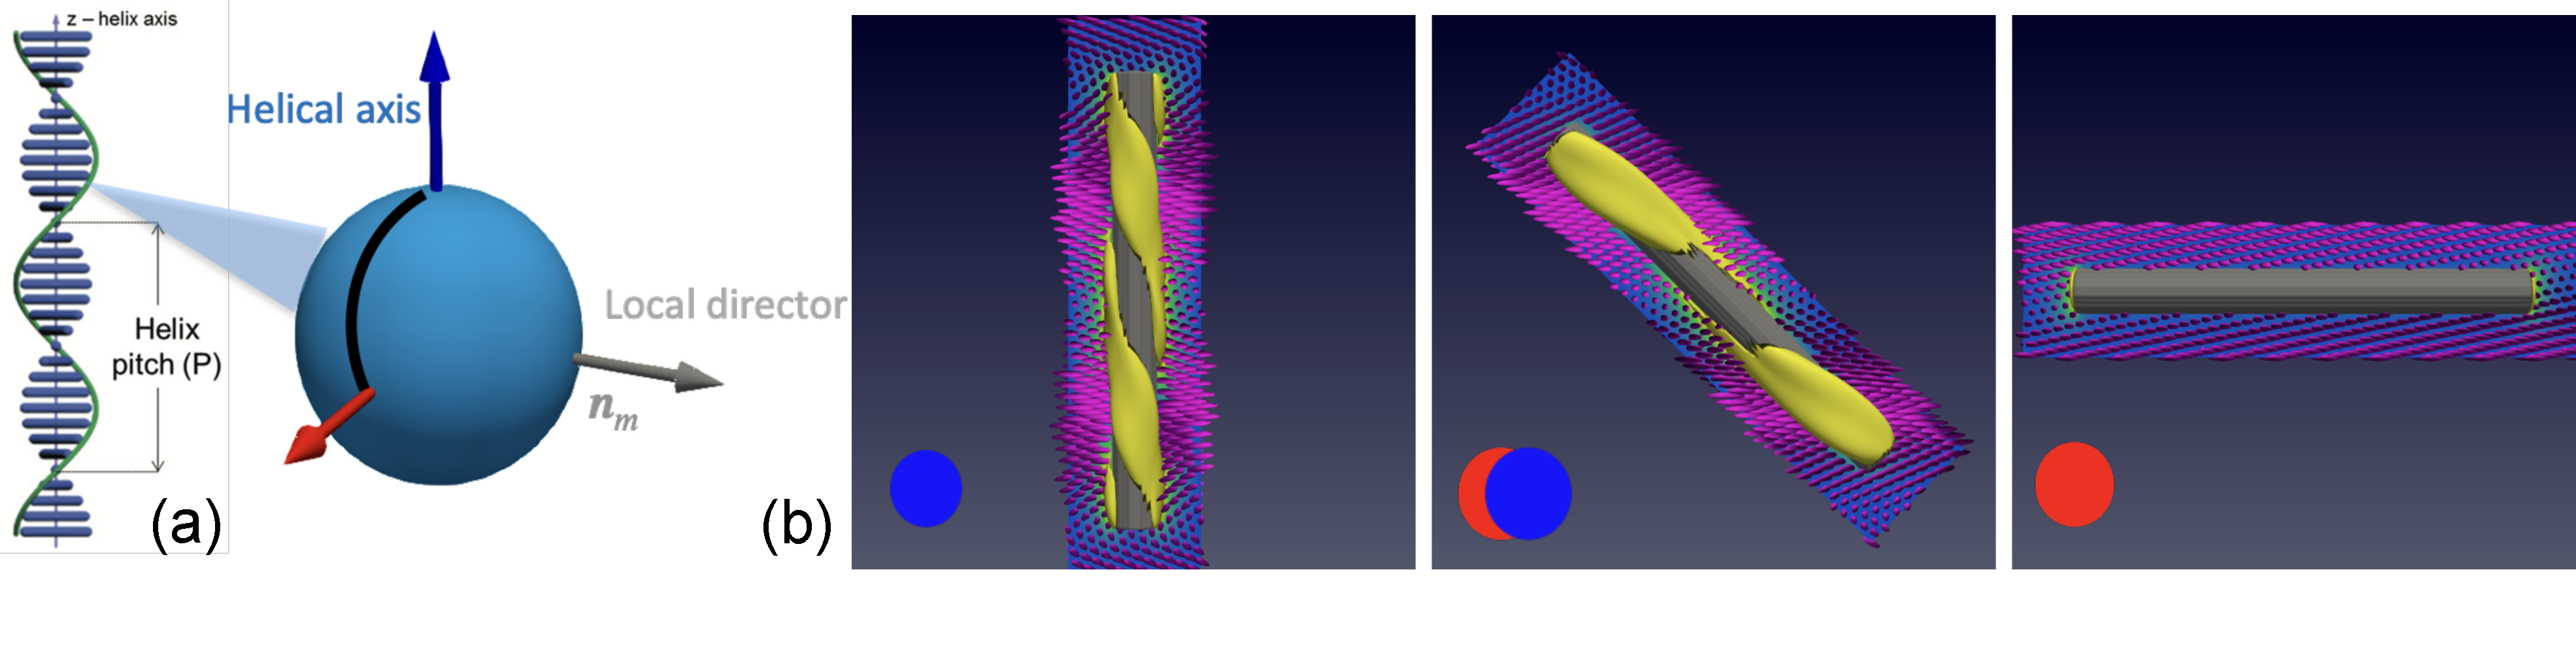
\includegraphics[width = \columnwidth]{figures/chapter-3/twisted_disclination}
	\caption{ (a) Local tripod of directions along the molecular helix. (b) Illustrations of a helical surface defect emerging around a colloidal cylinder at various orientations along the tripod, indicated by the colored dots. When the rod align along the blue helix axis a helically twisted disclination occurs. It is absent when the rod points along the red arrow. Picture courtesy of Jason Wu (University of Colorado, USA). }
	\label{twisdis}
\end{figure}




We will now attempt to quantify the twisted disclination effect by introducing an angular deviation $\Phi(\bfr)$ and express the helical host director as follows:
\beq
\bn_{s}(\bfr) = \bx \cos( q z + \Phi(\bfr_{\perp}))  + \by \sin (q z + \Phi(\bfr_{\perp}))
\label{nsebluee}
\eeq
with $\bfr$ denoting a 3D distance vector and $\bfr_{\perp}$  the lateral distance perpendicular to the helical axis $\bz$.  The total free energy of a colloidal rod inclusion aligned along the helical axis is given by the Rapini-Papoular surface anchoring term \eq{rapo} combined with the Frank elastic free energy in the presence of chirality:
\begin{align}
F &= \frac{1}{2} \int d \bfr \left [ K_{1} (\nabla \cdot \bn_{s})^{2}  + K_{2} (\bn_{s} \cdot \nabla \times \bn_{s} + q)^{2} \right . \nonumber \\
& \left . +   K_{3} (\bn_{s} \times \nabla \times \bn_{s})^{2} \right ]
-\frac{1}{2} W_{0} \oint d{\mathcal S}  (\bn_{s} \cdot \bn_{0}({\mathcal S}))^{2}
\end{align}
with $K_{1}$, $K_{2}$ and $K_{3}$ respectively denoting the splay, twist and bend elastic modulus.  The saddle-splay term surface elasticity reads:
\beq
F_{se} = -\frac{K_{24}}{2} \oint d{\mathcal S} \cdot \left ( \bn_{s} \nabla \cdot \bn_{s} +  \bn_{s} \times \nabla \times \bn_{s}\right )
\eeq
and is expected to have very little impact in the current geometry (cf. spherical colloidal inclusion).
The director twist is very weak on the typical range of the director deformations which should be comparable to the rod diameter $D$ rather than the rod length $L \gg D$. For simplicity, we assume the rod to be infinitely long and elastic distortions to occur only along the radial direction $\bfr_{\perp}$ Employing cylindrical coordinates $\Phi(\bfr_{\perp}) = \Phi (r, \vartheta ) $, expanding up to second order in $q$ and integration over the  we obtain for the  free energy  $ F_{el}$ per unit rod length:
\begin{align}
 \frac{F_{el}}{L} &=  \frac{1}{2} \int d  \bfr_{\perp} \left \{ \frac{K_{1}}{r^{2}} (1+ \partial_{\vartheta} \Phi)^{2} + K_{3} (\partial_{r} \Phi)^{2} \right . \nonumber \\
  & \left . + \frac{(qL)^{2}}{12} \Delta K  \left  [ \frac{1}{r^{2}} (1+ \partial_{\vartheta} \Phi)^{2} - (\partial_{r} \Phi)^{2} \right ] \right \}
  \label{felo}
  \end{align}
  where $\Delta K = K_{3} - K_{1} >0 $ denotes the difference between the bend and splay moduli. The elastic anisotropy turns out to be of crucial importance since the twist correction $\mathcal{O}(q^{2})$  vanishes in case of the one-constant approximation $K_{1} = K_{3} = K_{2} = K$.
Similarly, the surface anchoring free energy reads up to quadratic order in $qL \ll 1$:
\beq
  \frac{F_{s}}{L} =  -\frac{W_{0}}{2} \oint_{\mathcal{C}} d %
\vartheta \left \{ \cos^{2}(\vartheta - \Phi)  - \frac{(qL)^{2}}{12} \cos [2 ( \vartheta - \Phi)]  \right \}   \eeq
where $\mathcal{C}$ denotes the circular contour of the rod cross section with diameter $D$.
For weak distortions $\Phi \ll 1$ we linearize for $\Phi$ and obtain:
\beq
  \frac{F_{s}}{L} \approx \frac{F_{s}^{(0)}}{L} -\frac{W_{0}}{2} (1- \tfrac{1}{6} (qL)^{2}) \oint_{\mathcal{C}} d  \vartheta   \sin 2 \vartheta  \Phi
  \label{fsdist}
\eeq
The first term is the contribution for the {\em undistorted} director field previously analysed:
\begin{align}
  F_{s}^{(0)} &=  -\frac{LW_{0}}{2} \oint_{\mathcal{C}} d %
\vartheta \left \{ \cos^{2}\vartheta - \frac{(qL)^{2}}{12} \cos 2  \vartheta \right \} \nonumber \\
& \sim -\frac{\pi}{4} W_{0} LD
\label{sabasis}
\end{align}
which corresponds to \eq{usurf} for a homeotropic rod aligned perpendicular to the helical axis ($\theta = \delta = \pi/2$) in the large pitch limit $qL \ll 1$. The second term in \eq{fsdist} accounts for the change of surface anchoring free energy generated by the elastic distortions.
The change of elastic free energy induced by the twist follows from:
\begin{align}
 \Delta F_{\rm twist}^{(el)}  &\approx  \frac{1}{24} (qL)^{2} L \Delta K   \mathcal{F} [ \Phi_{0} ]
\end{align}
where $\Phi_{0}$ denotes the distortion angle for the {\em untwisted} system, and:
\beq
 \mathcal{F} [ \Phi_{0} ]  = \int d \bfr_{\perp}  \left [ \frac{1}{r^{2}} (1+ \partial_{\vartheta} \Phi_{0})^{2} - (\partial_{r} \Phi_{0})^{2} \right ]
 \label{fmans}
\eeq
is a dimensionless quantity measuring the extent of the surface disclination surrounding the cylinder. Applying the one-constant approximation which does not lead to qualitative changes in this context, we determine $\Phi_{0}$ from minimizing:
\begin{align}
 \frac{F_{el}(q=0)}{KL} &=  \frac{1}{2} \int d \bfr_{\perp}  \left \{ \frac{1}{r^{2}} (1+ \partial_{\vartheta} \Phi)^{2} + (\partial_{r} \Phi)^{2} \right \}
\end{align}
so that $(\delta F_{el} / \delta \Phi )_{\Phi = \Phi_{0}} = 0$ and $\ell_{s}  = K/W_{0}$ defines the (finite) surface anchoring extrapolation length.  Functional minimization of the free energy we obtain the Laplace equation in polar coordinates:
\beq
\partial_{r}^{2} \Phi_{0} + \frac{1}{r} \partial_{r} \Phi_{0}  + \frac{1}{r^{2}} \partial_{\vartheta}^{2}\Phi_{0} =0
\label{lapo}
\eeq
subject to the boundary conditions:
\begin{align}
\Phi_{0}( \infty, \vartheta ) &= 0 \nonumber \\
 \ell_{s} \partial_{r} \Phi_{0}(D/2, \vartheta) &= \tfrac{1}{2} \sin 2 \vartheta
\label{phioo}
\end{align}
with the latter denoting a Neumann boundary condition at the colloid surface imparted by surface anchoring contribution  \eq{fsdist}.
The result is a simple dipolar field:
\beq
\Phi_{0}(r , \vartheta ) = -\frac{D}{16 \ell_{s}} \left ( \frac{D}{2r}   \right )^{2} \sin 2 \vartheta
\eeq
Plugging this back into \eq{fmans} and integrating we find that the difference in elastic energy between the twisted (blue) and untwisted (red) case in independent of the surface anchoring extrapolation length $\ell_{s}$ and increases logarithmically with system size $\ell_{\rm max}$:
\beq
 \Delta F_{\rm twist}^{(el)} \sim  \frac{2 \pi }{24} (qL)^{2} L \Delta K  \ln \left ( \frac{2 \ell_{\rm max}}{ D} \right )
 \label{twidi}
 \eeq
 Taking $\ell_{\rm max} = L$ as typical size cut-off, $\Delta K \approx 4 pN$ we find that $\Delta F_{\rm twist}  \approx 280 k_{B}T$.
 %For the total elastic free energy for a rod with untwisted distortions we find:
%\beq
%F_{el}(q=0) = \pi K L \left \{ \frac{D^{2}}{256\ell_{s}^{2}} + %\ln \left ( \frac{2 \ell_{\rm max}}{ D} \right ) \right \}
%\eeq
%which is about $3.5 \times 10^{4}$ $k_{B}T$.
The change in surface anchoring free energy associated with a twist of the director distortions reads:
\begin{align}
  \Delta F_{\rm twist}^{(s)} &
  \sim - \frac{\pi W_{0}LD}{92} \frac{D}{ \ell_{s}}  (qL)^{2}
\end{align}
which is  negligible compared to the elastic contribution above so that the total distortion-induced free energy change reads $\Delta F_{\rm twist} \approx \Delta F_{\rm twist}^{(el)}$.






\subsection{Elastic distortions around a rod tilted away from the host director}

In order to complete our understanding of the strength of the elastic distortions surrounding the main section of the rod we now look at the case where the rod remains perpendicular to the helix axis but makes an oblique angle with respect to the host director (see \fig{fel}). Ignoring chiral twist we parameterize the host director field case within a Cartesian reference frame with the rod aligned along $\bz$:
\begin{align}
\bn_{s}(\bfr) = & \begin{pmatrix}
\cos \Phi(\bfr)  \cos \chi(\bfr)\\
\sin  \Phi(\bfr) \cos \chi(\bfr) \\
 \sin \chi(\bfr)
 \end{pmatrix}
\label{nseblueee}
\end{align}
 As before,  we ignore end effects and and express the spatial variation of the distortion angles in polar coordinates, i.e. $\Phi(r , \vartheta)$ and $\chi(r, \theta )$. In principle, the  Euler-Lagrange expressions emerging from minimizing the elastic free energy are strongly coupled and cannot be solved analytically even in the case of weak surface anchoring. We expect, however, that a tilted rod will mostly experience distortions along its main axis $\bz$, expressed by a non-zero $\chi$, while the director deviations $\Phi$ surrounding the lateral cross-section of the rod remain far less affected by the rotation. Then, we can pursue a hybrid route by `constraining $\Phi = \Phi_{0}$ to its solution for the perpendicular case \eq{phioo} and minimize the free energy only with respect to $\chi$.
Working out the one-constant elastic free energy and taking the functional derivative we find that $\chi$ satisfies the following non-linear partial differential equation:
\begin{align}
\partial_{r}^{2} \chi + \frac{1}{r} \partial_{r} \chi  + \frac{1}{r^{2}} \partial_{\vartheta}^{2} \chi & = -\frac{\sin 2 \chi }{2r^{2}}
\label{nlpde}
\end{align}
Corrections to the right-hand term are of order $\mathcal{O}(1/r\ell_{s})$ and can be neglected for weak surface anchoring $\ell_{s} \gg D$.
In order to accommodate a rotation of the rod axis with respect to the far field host director we define a rotation matrix:
\beq
\mathcal{R}(\delta)  = \begin{pmatrix}
\sin \delta  & 0 & - \cos \delta \\
0 & 1 & 0 \\
\cos \delta & 0 & \sin \delta \\
\end{pmatrix}
\eeq
such that $\delta = \pi/2$ reverts to the case where the far-field host  director is perpendicular to the rod axis. The boundary conditions then follow from the Rapini-Papoular surface anchoring energy where the surface normal $\bn_{0}$ is subject to rotation:
\begin{align}
F_{s} &= -\frac{W_{0}}{2} \oint d{\mathcal S}  [\bn_{s} \cdot  (\mathcal{R} ( \delta ) \cdot  \bn_{0}({\mathcal S}))]^{2} \nonumber \\
& = -\frac{  W_{0} L}{2 } \oint d \vartheta \cos^{2} \vartheta \sin^{2}(\delta - \chi(D/2, \vartheta))
\label{raporot}
\end{align}
from which we infer that at $\delta = \pi/2$ (red arrow) optimal surface anchoring is achieved  when the  distortion angle $\chi $ is zero, which leads back to \eq{sabasis}. For oblique orientations $0<\delta < \pi/2$, severe distortions are generated since the optimal anchoring angle at the rod surface $\chi_{\rm surf} \sim \delta - \pi/2$ is incompatible with the far-field condition $\chi(r \rightarrow \infty) =0$.
The boundary condition for $\chi$ are the following:
\begin{align}
\chi(  \infty, \vartheta ) = & 0 \nonumber \\
\ell_{s} \partial_{r} \chi(D/2, \vartheta ) = & - \frac{1}{2 } \cos^{2} \vartheta \sin [2(\delta - \chi(D/2, \vartheta))] \nonumber \\
& + D^{-1} \sin 2 \chi(D/2, \vartheta)
\end{align}
The latter condition tells us that the distortions will be independent of the tilt angle $\delta$ at infinitely weak surface anchoring ($\ell_{s} \rightarrow \infty$), as we expect.
Clearly, the non-linear nature of the above differential equation and the complicated boundary conditions do not allow for an analytical solution of the problem.


\begin{figure}
	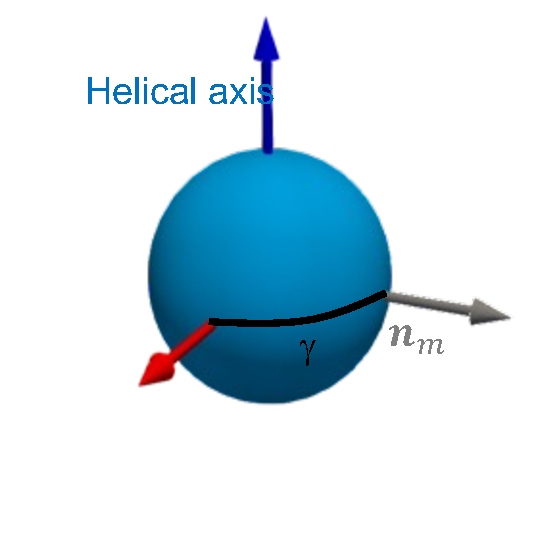
\includegraphics[width = .3\columnwidth]{figures/chapter-3/gamrods}
 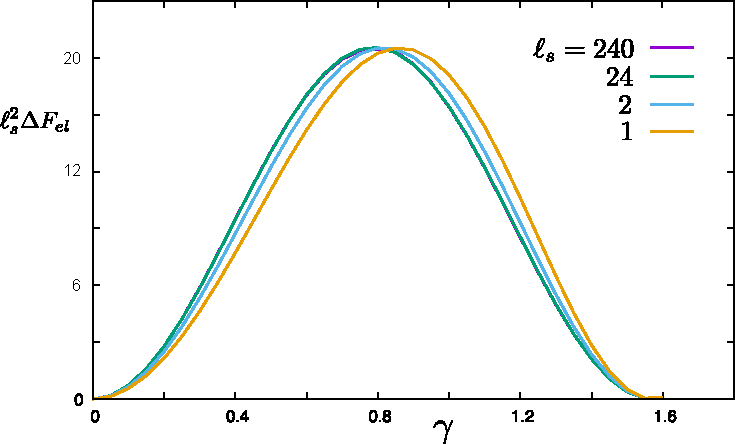
\includegraphics[width = .6\columnwidth]{figures/chapter-3/fel}
	\caption{Free energy associated with elastic distortions around a homeotropic rod tilted at an angle $\gamma$ away from the red arrow towards the molecular director (grey) at different surface anchoring extrapolation lengths $\ell_{s}$ (expressed in units of the rod diameter $D$).   }
	\label{fel}
\end{figure}




\subsubsection{Curvature-free rod cross-section}

A more tractable  way forward is to transform the above expressions into a Cartesian coordinate system, so that $\chi(x,y)$ with the far-field host director pointing along the $x$-axis. Basically, we  assume that the rod cross-section along which the director distortions are expected to occur can be described by a strip of length $L$ and $D \ll L$. Further, we define a tilt angle $\gamma = \delta - \frac{\pi}{2}$ (with $0<\gamma <\pi/2$) so that $\gamma =0$ corresponds to the most favorable case where the rod points perpendicular along the red arrow.  All distances are normalized in terms of $D$. The distortions are then described by the 2D Laplacian:
\beq
(\partial_{x}^{2} + \partial_{y}^{2}) \chi  = 0
\eeq
of which the general solution reads:
\beq
\chi(x,y) = \sum_{n=1}^{\infty} e^{-n \pi x } [ a_{n} \cos(n \pi y) + b_{n} \sin( n \pi y ) ]
\label{seriesxy}
\eeq
which vanishes in the far-field limit $\chi(x \rightarrow \infty) = 0$. The (Rapini-Papoular) surface anchoring free energy reads:
\begin{align}
\frac{F_{s}}{KL} = - \frac{1}{2 \ell_{s}} \int_{0}^{1} dy \cos^{2} (\gamma - \chi(0,y))
\end{align}
which translates into the following boundary condition at the surface of the strip located at $x=0$:
\beq
\ell_{s} \partial_{x} \chi(0,y) = \frac{1}{2 } \sin [ 2 (\gamma - \chi(0,y)) ]
\label{bcweak}
\eeq
Further, for symmetry reasons we require the distortion angle to be vanishing at both sides of the strip:
\beq
\chi(0, 0 ) = \chi(0, 1)  =0
\eeq
which implies that $a_{n} =0$. The coefficients $b_{n}$ need to be  resolved from:
\beq
n \pi b_{n} = \frac{1}{ \ell_{s}} \int_{0}^{1} dy \sin (n \pi y) \sin \left [ 2 \left (\gamma - \sum_{k=1}^{\infty} b_{k} \sin (k \pi y) \right ) \right ]
\label{bcnum}
\eeq
For small tilt angles $\gamma  \ll 1$  distortions are expected to be weak $\chi \ll 1$ so that we linearize $\sin 2 (\gamma - \chi ) \approx 2( \gamma  - \chi)$.
This enables us to resolve the coefficients analytically:
\beq
b_{n} =  \left ( \frac{1 - (-1)^{n}}{(n \pi)^{2}}\right ) \frac{\gamma}{\ell_{s}}
\eeq
The free energy increase induced by the elastic distortions is given by:
\begin{align}
\Delta F_{el} &= \frac{ \pi KL}{4} \sum_{n=1}^{\infty} n b_{n}^{2}
\label{dfelseries}
\end{align}
which in the linearized regime for small $\gamma$ gives a simple analytical result:
\begin{align}
\Delta F_{el} = \frac{7 KL}{8 \pi^{3}} \zeta(3) \left ( \frac{\gamma }{\ell_{s}} \right )^{2}
\label{felgg}
\end{align}
with $\zeta(3) \approx 1.2 $ a constant from the Riemann-Zeta function $\zeta(x)$. The surface anchoring free energy reads:
\begin{align}
F_{s} = - LDW_{0} \int_{0}^{1} dy \cos^{2} (\gamma - \chi(0,y))
\end{align}
Then, in the absence of elastic distortions and no tilt ($\gamma = 0$) the surface anchoring free energy would simply be $F_{s} = -LDW_{0}$ which only marginally differs from the result for the cylindrical case $F_{s} = -(\pi/4)LDW_{0}$.
Within the linearized regime for small tilt angles $\gamma \ll 1$  the change in surface anchoring free energy imparted by the elastic distortions is given by:
\begin{align}
\Delta F_{s} &\approx LDW_{0}  \int_{0}^{1} dy  (\gamma - \chi(0,y))^{2}  \nonumber \\
& \approx W_{0} LD  \left ( 1 + \frac{1}{48 \ell_{s}^{2}} - \frac{7  \zeta(3)}{ \pi^{3} \ell_{S}} \right) \gamma^{2}
\end{align}
This expression along with \eq{felgg} clearly reflects the basic trade-off between surface anchoring and elasticity in which the cost in elastic free energy is in part compensated by a reduction of the surface anchoring free energy (last term). The total free energy change for small tilt angles now reads:
\beq
\Delta  F_{\rm tot} \sim  W_{0} LD \left ( 1  - \frac{49 \zeta(3)}{8\pi^{3} \ell_{s}}  \right ) \gamma^{2} + \mathcal{O}(\gamma^{2}/\ell_{s}^{2})
\label{ftiltcorr}
\eeq
Let us now compare our results with the simple Rapini-Papoular expression \eq{usurf} in the {\em absence} of elastic distortions. Taking $\theta=\pi/2$ and expanding for small $\gamma $ we find:
 \beq
 \Delta  F_{\rm tot}^{(RP)} \sim \frac{\pi}{4} W_{0}LD \gamma^{2}
\eeq
Disregarding the trivial curvature prefactor $\pi/4$ in the last expression, we find that the impact of the elastic distortions is rather marginal, since the correction term in  \eq{ftiltcorr} is less than 1 $k_{B}T$. Numerical resolution of \eq{bcnum} reveals that weak elastic distortions  occur mostly when the rod is at an oblique angle $\gamma = \pi/4$.
This is illustrated in \fig{fel} for a number of different anchoring strengths expressed by the extrapolation length $\ell_{s}$.

Now that we have established that distortions remain weak at any angle $\gamma$ for large enough extrapolation length $\ell_{s}  \gg 1$ we may explore an alternative route to quantifying $\chi$ by linearizing the boundary condition \eq{bcweak} for $\chi \ll 1$:
\beq
\ell_{s} \partial_{x} \chi(0,y)\approx \frac{1}{2 } \sin ( 2 \gamma) - \chi(0,y) \cos (2 \gamma )
\label{bcweak}
\eeq
From which the coefficients are easily established:
\beq
b_{n}  = \frac{\sin ( 2 \gamma )}{\cos(2 \gamma) - n \pi \ell_{s}} \left ( \frac{1-(-1)^{n}}{n \pi}\right )
\eeq
The corresponding elastic free energy then follows from the summation in \eq{dfelseries} and the results agree with the ones shown in \fig{fel}.







\subsection{Effective orientational potential of a LC rod}

Gathering the findings of the previous paragraphs we revisit the realigning potential acting on each rod. The total external potential is given by the bare Rapini-Papoular contribution \eq{usurf} for the undistorted host director plus the free energy contributions from elastic distortions:
\beq
U_{\rm rod} (\theta, \delta) \sim  F_{s}(\theta, \delta)  + \Delta F_{\rm dist}(\theta, \delta)
\eeq
Since the distortion term cannot be resolved for any rod orientation but only for cases when the rod is aligned along the principal Cartesian axes of the host frame we use the following interpolation form:
\begin{align}
\Delta F_{\rm dist} (\theta, \delta)  \sim & \Delta F_{\rm twist} \cos^{2} \theta  + \Delta F_{\rm tilt} \sin^{2} \theta \cos^{2} \delta
\end{align}
in terms of the two principal elastic  contributions;  $\Delta F_{\rm tilt} = F(\textrm{grey}) - F(\textrm{red})$ associated with tilting  the rod away from the red arrow and $\Delta F_{\rm twist}$ [\eq{twidi}] the energy cost associated with twisting of the surface disclination wrapped along the main part of the cylinder. From the analysis in the previous paragraphs we  found that $\Delta F_{\rm twist} = \mathcal{O}(10^{2} k_{B}T)$ whereas elastic distortions due to tilting are very weak $\Delta F_{\rm tilt} < k_{B}T$ and may, in fact, be neglected all together for the weak anchoring regime.  The  elastic energy is minimal (zero) when the rods align along the red arrow ($\theta = \pi/2$ and $ \delta= \pi/2 $) as observed in experiment.

At infinitely low rod concentrations, the order parameters $S$ and $\Delta$ defined within the frame of the  molecular host (\eq{s2} and \eq{d2}) are readily computed from the Boltzmann factor
  $f( \bhu ) = \mathcal{N} \exp ( - \beta  U_{\rm rod} (\delta, \theta)   ) $.
An overview of the results as a function of the anchoring strength $\bar{w} = \beta W_{0} LD$ is given in \fig{ww}. The best correspondence with experimental data for homeotropic rods listed in Table 3.1 is found for $ \bar{w} \sim 6 k_{B}T$ which corresponds to a surface anchoring  amplitude of about $W_{0}\sim 6 \times 10^{-7} J/m^{2}$.


\begin{figure}
	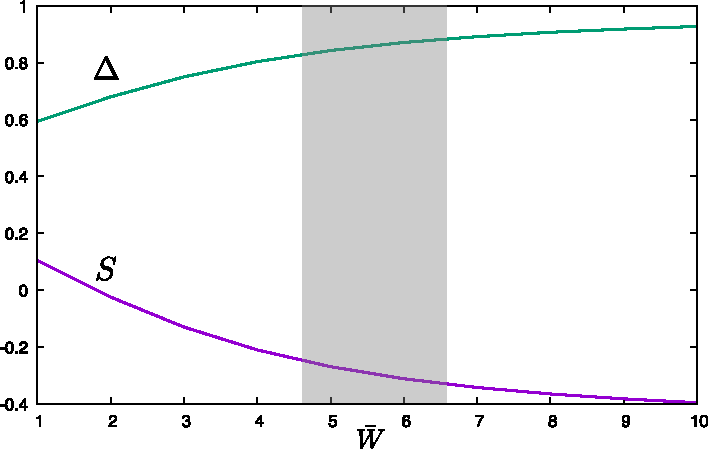
\includegraphics[width = .8\columnwidth]{figures/chapter-3/wwmans}
	\caption{ Colloidal nematic order parameters measured within the molecular frame as a function of
the surface anchoring amplitude $\bar{w} = W_{0}LD$. The experimentally relevant region is indicated in grey. }
	\label{ww}
\end{figure}



The typical energy scale related to the twisted disclination effect can be gleaned from the the orientational distribution of the colloidal particles that have been measured in experiment.  From these, we can identify a standard Gaussian ${\rm FWHM} =2.355/\sqrt{2 \Delta F_{\rm twist}}$. This subsequently gives $\Delta F_{\rm twist} \approx 22 k_{B}T$ for homeotropic rods with  $L  = 1.7 \mu m $  and $\Delta F_{\rm twist} \approx 76 k_{B}T$  for the longer rods  with $L  = 3 \mu m $ suggesting that, in both cases, the thermal motion of the rods is assuredly insufficient to overcome the energy barrier between the $\tau$ and $\chi$ alignment directions. The values are in qualitative agreement with the prediction from our analytical model \eq{twidi} where $\Delta F_{\rm twist} \propto L^{3}$ suggests the energy to indeed be quite sensitive to the colloidal rod length. The actual values from  \eq{twidi}, however, should be considered as an upper bound for $\Delta F_{\rm twist}$ mainly because in our model the local nematic order parameter of the host is constrained at its far-field bulk value and is not allowed to relax in regions where director distortions are the largest, as observed in the experiment and simulations. 








\subsection{Short-pitch cholesteric hosts}


 At much short pitches,  comparable to the disc diameter, fluctuations in $\delta$ are greatly facilitated and the local minimum of $U_{\rm disc}$ eventually switches over to $\delta = \pi/2$ suggesting  discs  preferentially aligning perpendicular to the director and helical axis.  Taking the Rapini-Papoular contribution \eq{usp} as the main contribution for the weak surface anchoring regimes considered here we can extract  nematic order parameters associated with such a crossover.  The results, shown in \fig{disop}, clearly exhibit a sharp transition from uniaxial to biaxial order at a critical pitch of about $qD \approx 3.8$ which, taking $D =2 \mu m$ would correspond to cholesteric pitch of about $p \approx 3.3 \mu m$.



\begin{figure}
	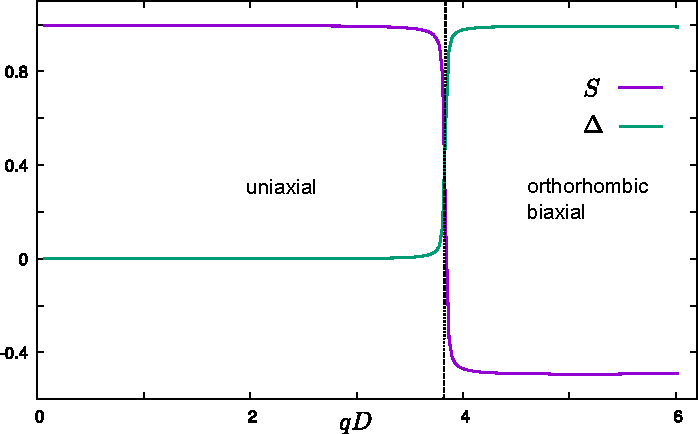
\includegraphics[width =  .8\columnwidth]{figures/chapter-3/discubx}
	\caption{Nematic order parameters of discs with weakly homeotropic surface anchoring immersed in a cholesteric host with variable pitch $qD$. A crossover from uniaxial to orthorhombic biaxial local order occurs at around $qD \approx 3.8$.  }
	\label{disop}
\end{figure}



\subsection{Elastic distortions around a disc}

Ignoring elastic distortions we find that discs with homeotropic surface anchoring tend to orient along the grey axis, as observed in experiment (see Table 3.1). This is the obvious optimal situation that incurs the least amount of elastic distortions, compared to the other principal directions in which cases the disc surface would experience strongly unfavorable tangential surface ordering. However, even when the disc normal is aligned along the local nematic director  there are, however, local mismatches between the far-field and preferred surface director due to the weak twisting of the host director perpendicular to the disc normal (which occurs along the red axis) and when the rod normal fluctuates away from this axis. The elastic distortions are expected to be weak but they will become more outspoken at shorter pitches.  It is instructive to compute the extent of these distortions along the lines of our previous analysis for rods. Let us consider an infinitely thin disc with its normal restricted to lie in the $xy$-plane at an angle $\delta$ away from the optimal direction indicated by the grey arrow ($x$-axis). The principal directions are indicated by the tripod in \fig{discel} with the $xy$-plane corresponding to the one spanned by the red and grey arrows. We assume weak elastic distortions $\chi$  developing in the $xy$-plane.  Defining a host director $\bn_{s} = (\cos \Phi(x,y),
\sin \Phi(x,y) , 0)$ we find,  assuming  elastic isotropy,  that the distortions are described by the Laplace equation:
\beq
(\partial_{x}^{2} + \partial_{y}^{2}) \Phi  = 0
\eeq
The effect of a twisting host director is accounted for in the surface anchoring free energy:
\begin{align}
F_{s} &=  -\frac{W_{0}}{2} \oint d{\mathcal S}  [\bn_{s} \cdot  (\mathcal{R} (qz + \psi) \cdot  \bn_{0}({\mathcal S}))]^{2}
\label{raporotdisc}
\end{align}
where ${\mathcal S} $ parameterizes the face of the disc (as previously we ignore finite thickness effects for discs with $D \gg L$) and $\bn_{0} = (1,0,0)$ indicating homeotropic anchoring along the surface normal. The rotation matrix reads:
\beq
\mathcal{R}( qz )  = \begin{pmatrix}
\cos qz  & -\sin qz  & 0 \\
\sin qz & \cos qz & 0 \\
0 & 0 & 1 \\
\end{pmatrix}
\eeq
A key distinction with the rod case is that the distortions are not uniform across the disc surface but depend on the location of the surface element with respect to the helical axis.  It is convenient to divide the disc surface into infinitely thin strips, with each surface element on the strip being equidistant from the centre-of-mass along the twist direction ($z$-axis) thus experiencing the same degree of elastic distortions.

For notational brevity, we implicitly normalize all lengths in units of the disc diameter $D$ and parameterize the disc surface in terms of $y = \tfrac{1}{2} \cos \alpha$ and $z = \tfrac{1}{2} \sin \alpha$ with $-\pi < \alpha <  \pi$. Each strip then has length $L_{s} = \cos \alpha$ and thickness $D_{s} = \tfrac{1}{2} \cos \alpha d \alpha$ and surface $ds = L_{s}D_{s} $. The surface anchoring free energy of an arbitrary strip with surface $ds$ and centre-of-mass distance $z$ then reads:
\begin{align}
F_{s}^{\rm strip}  &= -W_{0} [\cos (\Phi(0,y) - qz -\delta )]^{2} ds
\label{sadisc}
\end{align}
The boundary condition at the strip the disc equator ($\alpha=0)$ reads:
\begin{align}
\Phi(  \infty, 0 ) & =  0 \nonumber \\
\ell_{s} \partial_{x} \Phi(0, y ) & =   -\frac{1}{2 }   \sin [2 ( \Phi(0,y) - qz - \delta ) ] \nonumber \\
& \approx \frac{1}{2} \sin [2(qz + \delta)]  - \cos [2 (qz + \delta)] \Phi(0,y)
\label{bcdisc1}
\end{align}
where we take $0<y<1$ for convenience. The distortions should be symmetric at the edges ($\Phi (0,0)  = \Phi (0, 1)$)
and the solution of the Laplace equation is the same as for the rod considered in Section 3.4.2:
\beq
\Phi(x,y) = \sum_{n=1}^{\infty} e^{-n \pi x }  b_{n} \sin(n \pi y)
\label{seriesxy}
\eeq
Fortunately, the boundary condition \eq{bcdisc1} is the same as the linearized one  for the rod (\eq{bcweak}) upon replacing $\gamma \rightarrow qz + \psi $. The same goes for the coefficients which now read:
\beq
b_{n}  = \frac{\sin [ 2 (qz+ \delta)  ]}{\cos[2 (qz + \delta)] - n \pi \ell_{s}} \left ( \frac{1-(-1)^{n}}{n \pi}\right )
\label{bnscenario1}
\eeq
Given that  $q$ and $-q$ do not give equivalent results we conclude that the distortions created near the disc surface carry a distinct {\em chiral signature} imparted by the chirality of the host LC, in agreement with simulations results from the group of I. Smalyukh depicted in \fig{chirdisc}. The nature of the imprint depends on the twist angle $\psi$ between the disc normal and the grey axis.
We further deduce that the distortions vanish at infinitely weak surface anchoring ($\ell_{s} \rightarrow \infty$) and in the absence of twist and tilting ($q=0$ and $\psi=0$), as we expect. The elastic free energy for the total disc is given by:
\beq
\Delta F_{el} = \frac{\pi KD}{4}  \int_{-\pi/2}^{\pi/2} d \alpha \cos \alpha \sum_{n} n b^{2}_{n}
\eeq
which may be evaluated as a function of the angle $\psi$ between the disc normal and the grey axis taking the surface anchoring extrapolation length (in units $D$) to be about $\ell_{s} \approx 3$.
The change in surface anchoring free energy induced by the distortions follows from linearizing \eq{sadisc} and integrating over all strips:
\begin{align}
\Delta F_{s}  &= \frac{W_{0}D^{2}}{2} \int_{-\pi/2}^{\pi/2} d \alpha \cos^{2} \alpha \sin[2(qz + \delta)] \nonumber \\
&\times \sum_{n} b_{n}  \left ( \frac{1-(-1)^{n}}{n \pi}\right )
\label{sadiscseries}
\end{align}
We reiterate that $z$ depends on the angle $\alpha$ via $z = \tfrac{D}{2} \sin \alpha$.
\begin{figure}
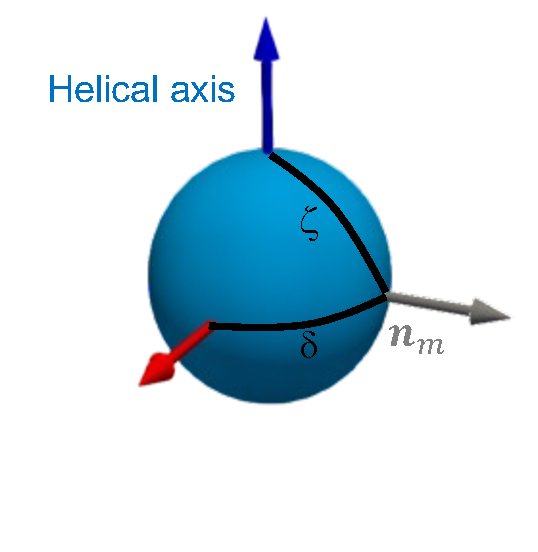
\includegraphics[width = 0.4 \columnwidth]{figures/chapter-3/deldisc}
	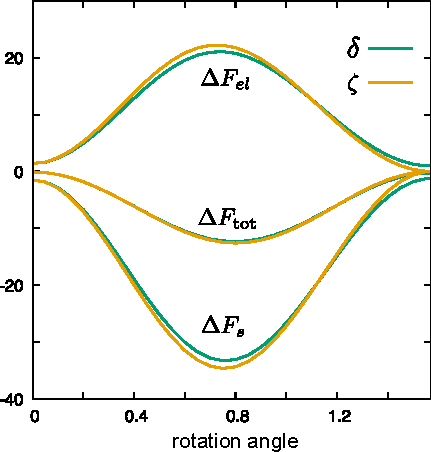
\includegraphics[width = 0.5 \columnwidth]{figures/chapter-3/discelastic}
	\caption{ Distortion free energies (in units $k_{B}T$) around a disc immersed at an angle $\delta$ or $\zeta$ with the local host director. The distortion free energies remain relatively weak for all $\delta$, but are most pronounced at oblique angles $\delta \sim \pi/4$. Parameters are based on the experimentally relevant situation: $qD =0.4$ and $\ell_{s}/D = 3$ ($W_{0} = 10^{-6} J/m^{2}$). }
	\label{discel}
\end{figure}






\begin{figure}
	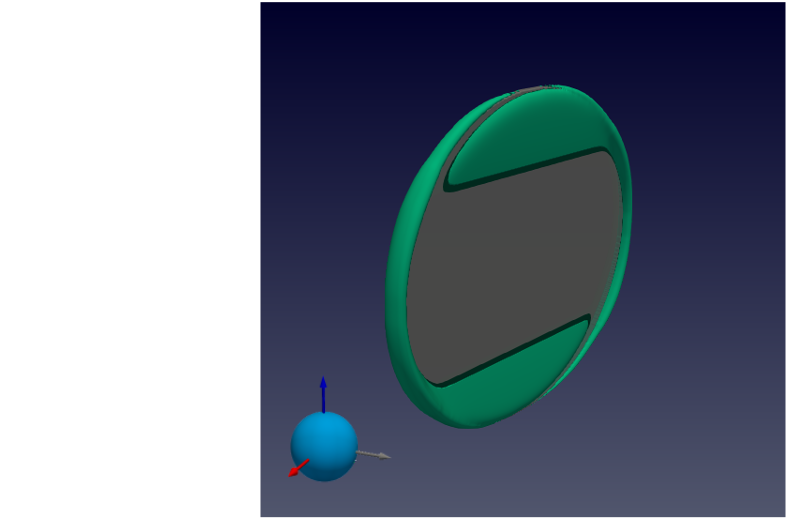
\includegraphics[width =  .7\columnwidth]{figures/chapter-3/chiraldisc}
	\caption{Computer simulation snapshot demonstrating the chiral defect structure (colored in green) around a disc with hometropic surface anchoring immersed in a molecular cholesteric host LC. Picture courtesy of Jason Wu (University of Colorado, USA). }
	\label{chirdisc}
\end{figure}






We  finish our analysis by considering the case where the disc normal rotates within the $xz$-plane over an angle $\zeta = \tfrac{\pi}{2} - \theta$ away from the molecular director (grey) as indicated in \fig{discel}. In this situation, the tilting will generate additional weak distortions  across the $z$-direction that we denote by the angle $\chi$. The spatially-dependent host director now reads:
\begin{align}
\bn_{s}(\bfr) = & \begin{pmatrix}
\cos \Phi(\bfr)  \cos \chi(\bfr)\\
\sin  \Phi(\bfr) \cos \chi(\bfr) \\
 \sin \chi(\bfr)
 \end{pmatrix}
\label{nseblue}
\end{align}
with $\bfr = ( x,y )$. As before each distortion angles obeys the Laplace equation in the $xy$-plane:
\begin{align}
(\partial_{x}^{2} + \partial_{y}^{2}) \Phi  &= 0 \nonumber \\
(\partial_{x}^{2} + \partial_{y}^{2}) \chi  &= 0
\end{align}
The surface anchoring free energy now takes the following form:
\begin{align}
F_{s} &=  -\frac{W_{0}}{2} \oint d{\mathcal S}  [\bn_{s} \cdot  (  \mathcal{R}_{\zeta} \mathcal{R} (qz) \cdot  \bn_{0}({\mathcal S}))]^{2}
\label{raporotdisc2}
\end{align}
where the matrix $\mathcal{R}_{\zeta}$ describes a rotation of the disc normal within the $xz$-plane:
\beq
\mathcal{R}_{\zeta}=
\begin{pmatrix}
\cos \zeta & 0 & \sin \zeta \\
0 & 1 & 0 \\
-\sin \zeta & 0 &  \cos \zeta \\
\end{pmatrix}
\eeq
Analogous to the previous case, we may derive boundary conditions from linearizing $F_{s}$ for weak distortions $\Phi \ll 1$ and $\chi \ll1$. Plugging in the general solution [\eq{seriesxy}] and defining $b_{n}$ as the distortion modes pertaining to $\Phi(x,y)$ and $d_{n}$ as those for $\chi(x,y)$ we find that both distortion angles are intricately coupled, as expected:
\begin{align}
b_{n} &=  c_{n} \cos \zeta \sin (2 q z) \nonumber \\
d_{n} & = c_{n} \sin (2 \zeta) \cos^{2} (q z)
\end{align}
From these we immediately assert  the most basic scenarios; both distortions vanish for a disc in an achiral host ($q=0$) at zero tilt ($\zeta=0$), whereas at nonzero tilt angle only $\chi(d_{n}) $ is nonzero. For a disc immersed in a chiral host ($q \neq$) at zero tilt ($\zeta =0$) we recover the previous scenario with $\Phi(b_{n})$ given by \eq{bnscenario1} and $\chi(d_{n}) =0$]. Both distortion angles are expected to be nonzero in case the disc normal is tilted away from the local director of the chiral host. The common prefactor reads:
\beq
c_{n} = \frac{ 2\left ( \frac{1-(-1)^{n}}{n \pi}\right )}{1 + 2\ell_{s} n \pi  -\cos( 2 \zeta) - 2 \cos^{2} \zeta \cos (2 q z)}
\eeq
The change in elastic free energy is a simple superposition of amplitudes:
\beq
\Delta F_{el} = \frac{\pi KD}{4}  \int_{-\pi/2}^{\pi/2} d \alpha \cos \alpha \sum_{n} n \left ( b^{2}_{n} + d_{n}^{2} \right )
\eeq
The contribution arising from the host chirality turns out zero for symmetry reasons:
\begin{align}
 \Delta F_{\rm chiral} &=  K q \int d \bfr \partial_{y} \chi (x,y) =0
\end{align}
which is easily inferred from inserting the expansion \eq{seriesxy} and integrating over $y$.
The reduction in surface anchoring free energy caused by the distortions  $\Phi$ is as follows:
\begin{align}
\Delta F_{s, \Phi} = W_{0}D^{2} \cos \zeta  \int_{-\pi/2}^{\pi/2} d \alpha \cos^{2} \alpha \sin (2 qz) \nonumber \\
\times \sum_{n} b_{n} \left ( \frac{1-(-1)^{n}}{n \pi}\right )
\end{align}
supplemented with a similar contribution accounting for the distortions $\chi$:
\begin{align}
\Delta F_{s, \chi} = W_{0}D^{2} \sin( 2 \zeta ) \int_{-\pi/2}^{\pi/2} d \alpha \cos^{2} \alpha  \cos^{2} (qz) \nonumber \\
\times \sum_{n} d_{n} \left ( \frac{1-(-1)^{n}}{n \pi}\right )
\end{align}
Note the surface anchoring is always negative and should outweigh the cost in elastic free energy. The results in \fig{discel} demonstrate that elastic distortions are most developed at oblique orientations, and do not strongly depend on the direction along which the disc is tilted.

\begin{figure}
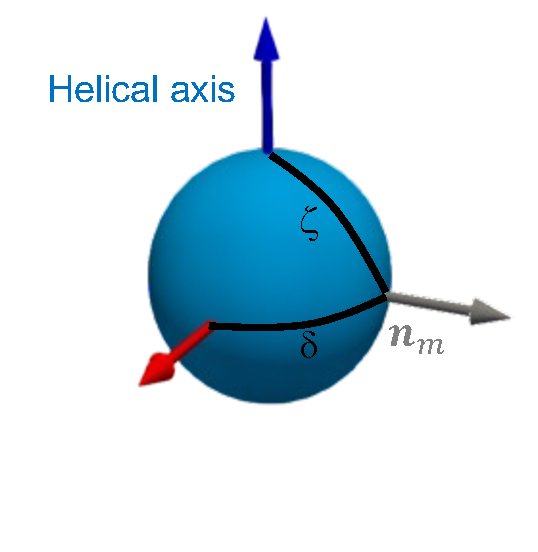
\includegraphics[width = 0.25 \columnwidth]{figures/chapter-3/deldisc}
	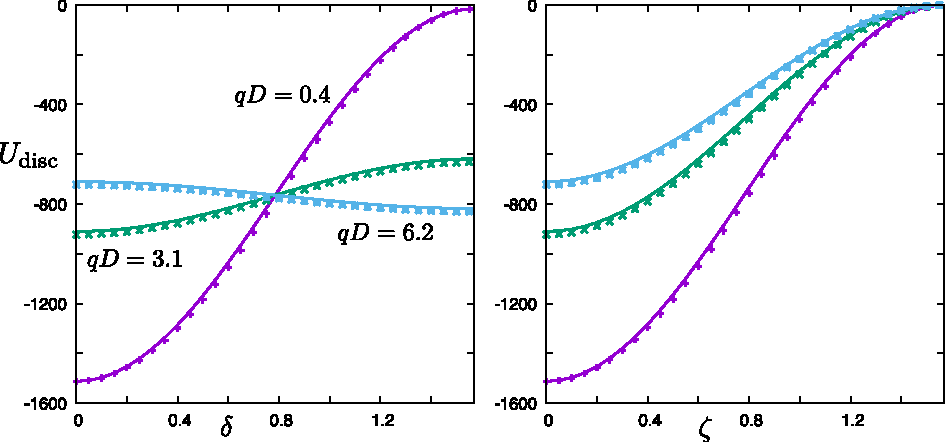
\includegraphics[width = 0.7 \columnwidth]{figures/chapter-3/udisc}
	\caption{Free energy of a colloidal disc with weakly homeotropic surface anchoring immersed in a cholesteric host with pitch $qD$ as a function of its orientation with respect to the local cholesteric director.  Solid lines correspond to surface anchoring only  [\eq{usp}], while the symbols denote the surface anchoring free energy including weak elastic distortions around the disc.  }
	\label{udisc}
\end{figure}

 If we now reconsider the {\em total} alignment potential for discs accounting for corrections derived above we conclude that the ordering of the discs is hardly affected by the distortions. The free energy changes are typically several tens of $k_{B}T$ which is about two orders of magnitude smaller than the typical Rapini-Papoular surface anchoring free energy $ W_{0} D^{2} $ which is about 1500 $k_{B}T$. Discs experiencing weak surface anchoring with  a cholesteric host with large pitch ($qD <1$)  will therefore simply follow the local molecular director with thermal fluctuations around the optimum angle being strongly suppressed. The considerable penalty incurred  by angular fluctuations away from the local cholesteric director is demonstrated in \fig{udisc} for a number of different host pitches. The elastic distortions around the disc surface lead to a systematic reduction of the free energy, as expected, but their effect on the realigning properties is rather marginal. At short pitches, the disc takes ona preferred angle $\delta = \pi/2$ and aligns along the red arrow, leading to pronounced local biaxial order as highlighted in \fig{disop}. 


 


\section{Conclusions}


We have  demonstrated that immersing uniaxial, non-chiral colloidal rods and disks into a low-molecular-weight cholesteric liquid crystal host leads to emergent biaxial order that we identify by combining experiment with numerical simulation and analytical theory. Unlike the previously studied case of hybrid molecular-colloidal biaxial phases \cite{liu2016,mundoor2021,mundoor2018}, we observe multi-level biaxial symmetry-breaking at ultralow colloidal content where colloid-colloid interactions are negligible. By exploring a variety of colloidal shapes and surface anchoring symmetries we report biaxial order emerging at three distinct levels. First, molecular director distortions develop around each colloid which, although being of marginal extent because of weak surface anchoring conditions, display a distinct two-fold signature imparted by the cholesteric host. Second, the orientational distribution of the colloids around the local cholesteric director is demonstrated to adopt a clear biaxial signature, and the response of the corresponding biaxial order parameter is found to depend non-trivially upon the surface anchoring strength as well as the ratio of the cholesteric pitch and the principal colloidal dimension (rod length or disk diameter). 

A particularly striking manifestation of biaxial symmetry-breaking is encountered for thermotropic cholesterics doped with colloidal rods with homeotropic surface anchoring. Driven by a combination of surface anchoring forces and an energy penalty incurred by twisting a weakly developed surface disclination along the rod main axis, these rods have a strong tendency to align perpendicular to both the helical axis and the local cholesteric director, thus imparting a two-fold $D_{2h}$ orientational symmetry onto the hybrid system at each point along the cholesteric helix.
By means of a simple mean-field theory based on the Rapini-Papoular surface anchoring energy combined with an analytical elasticity theory addressing the corresponding elastic distortions incurred by the presence of the colloids, we have revealed that the multi-level expression of emergent biaxiality in our systems is essentially a single-colloid effect that can be achieved in a wide variety of cholesteric systems doped with non-isotropic colloids. The next chapter will deal with possible scenarios that could arise when the colloid concentration is no longer negligible, and direct correlations between the colloids interfere with the surface anchoring effects discussed in this chapter. 




\clearpage